%------------------------------------------------------------------------
%Editar Diplomado
\hypertarget{cv:GestionarPrecondiciones}{\section{Gestionar Pre/Postcondiciones}} \label{sec:GestionarPrecondiciones}

	Esta funcionalidad le permitirá las acciones necesarias para controlar las precondiciones y postcondiciones pertenecientes a un caso de uso y visualizarlos en una tabla en el caso de uso sobre el que se está operando y solicitar el registro de uno nuevo.

		\subsection{Procedimiento}

			%Pasos de procedimiento
			\begin{enumerate}
				
			\item Ingrese a un proyecto existente desde la pantalla \ref{fig:GestionarProyectosColaborador}.
			
			\item Oprima el botón \IUCondiciones{} de algún registro existente de la pantalla \ref{fig:GestionarCU} ''Gestionar Casos de Uso''.
	
			\item Se mostrará la pantalla \ref{fig:GestionarPrePostcondiciones} ''Gestionar Pre/Postcondiciones''.

			%Pantalla
			\begin{figure}[htbp!]
				\begin{center}
					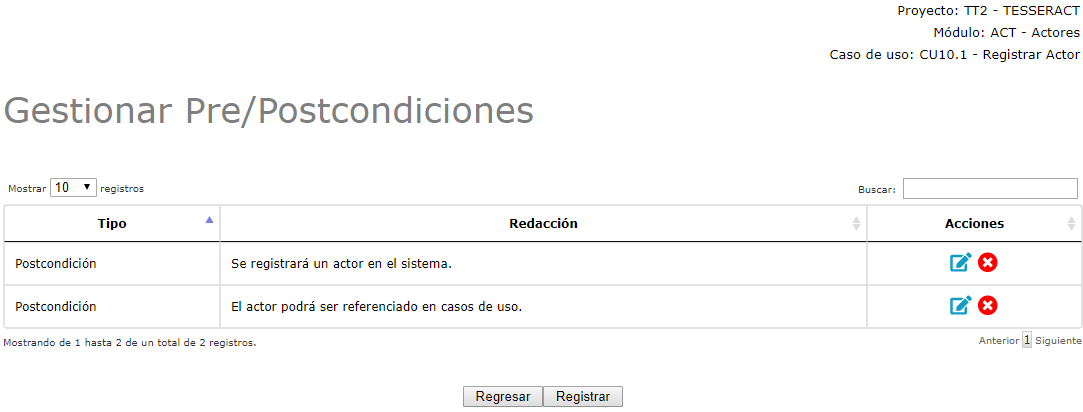
\includegraphics[scale=0.6]{roles/lider/casosUso/precondiciones/pantallas/IU6-1-2gestionarCondiciones}
					\caption{Gestionar Pre/Postcondiciones}
					\label{fig:GestionarPrePostcondiciones}
				\end{center}
			\end{figure}
		
				\item Seleccione la operación que desea realizar:
			
			Para (\hyperlink{cv:registrarCondicion}{Registrar}) dé clic en el botón \IURegistrar.
			
			Para (\hyperlink{cv:modificarCondicion}{Modificar}) dé clic en el botón \IUEditar de alguna condición ya registrada.
			
			Para (\hyperlink{cv:eliminarCondicion}{Eliminar}) dé clic en el icono \IUBotonEliminar{} de alguna condición ya registrada.
			
			\end{enumerate}